% OrbitGraph SDN design section.

\section{OrbitGraph Design}
\label{sec:orbitgraph}

LEO constellations are naturally modeled as \emph{time-varying weighted
graphs}: satellites and ground stations are vertices, inter-satellite and
ground--satellite links are edges whose weights shift as orbital geometry
changes~\cite{seong:topological-design:1995,kassing2020exploring,handley:ground-relays:2019}.
Distributed link-state protocols such as OSPF~\cite{sidhu:ospf:1993} must
discover each mutation through hello timeouts and LSA flooding before forwarding
stabilizes, which creates multi-second black holes at ground--satellite (GSL)
handovers in our baseline (Section~\ref{sec:experiments}).
OrbitGraph takes a graph-centric, software-defined view: a centralized
controller reads the same orbital snapshots that drive the emulator, computes
shortest paths on the current graph, and programs the kernel forwarding
information base (FIB) on each node.
Because topology changes are known in advance from ephemeris-driven delay
matrices~\cite{lai2023starrynet}, the controller can push route \emph{deltas}
before links are torn down---a capability unavailable to reactive distributed
routing~\cite{gregory:satellite-routing:2022,pam:opspf:2019}.

OrbitGraph splits the network into a \emph{control plane} (central controller)
and a \emph{data plane} (Linux kernel forwarding in StarryNet containers).
No OpenFlow switch is required: static routes installed via \texttt{ip route}
constitute the programmed data plane, matching how operator SDN deployments
often push FIB state to edge routers.

\subsection{Dynamic graph model}

\begin{figure}[!t]
  \centering
  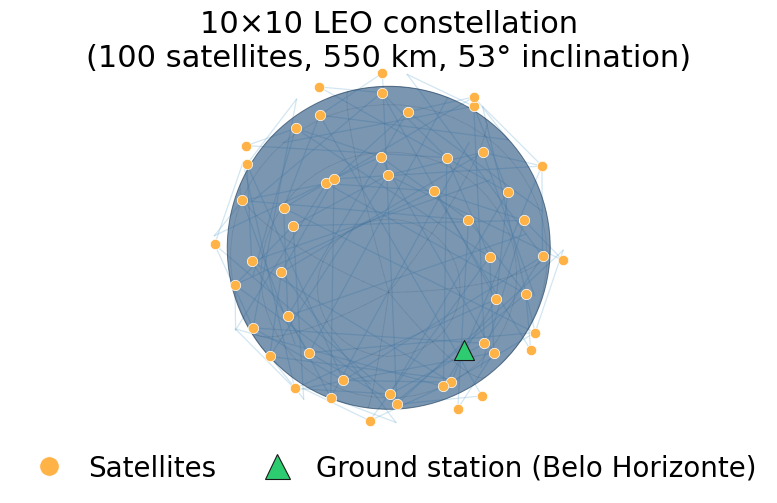
\includegraphics[width=\linewidth]{figures/constellation_10x10.png}
  \caption{Representative $10{\times}10$ Walker constellation at 550\,km and
    53$^\circ$ inclination (100 satellites, +Grid ISLs; ground station shown:
    Belo Horizonte).
    This is the largest grid in our scaling study; smaller grids use the same
    topology class with fewer orbital planes and satellites per plane.}
  \label{fig:constellation-10x10}
\end{figure}

At emulation second~$t$, StarryNet provides an $N \times N$ delay matrix
$D_t = (d_{ij})$ whose entries are one-way propagation delays (milliseconds)
between nodes $i,j \in \{1,\ldots,N\}$, derived from SGP4 orbital state.
We construct an undirected weighted graph
\begin{equation}
  G_t = \bigl(V,\, E_t,\, w_t\bigr),
  \label{eq:graph}
\end{equation}
where $V$ is the set of satellite and ground-station nodes (Fig.~\ref{fig:constellation-10x10}),
\begin{equation}
  E_t = \bigl\{ \{u,v\} \subseteq V \;\big|\;
         d_{uv} > \tau \bigr\},
  \label{eq:edges}
\end{equation}
with link threshold $\tau = 0.01$\,ms filtering zero-delay (absent) links, and
\begin{equation}
  w_t(u,v) = d_{uv}.
  \label{eq:weight}
\end{equation}
Damaged satellites (100\% loss during failure injection) are removed from $V$
for the duration of the fault, yielding $G_t^{\mathrm{fault}} \subseteq G_t$.

OrbitGraph treats each routing event---initialization, delay refresh, damage
recovery, or GSL handover---as a \emph{snapshot} indexed by~$t$.
The controller loads $D_t$, builds $G_t$, and derives a forwarding policy for
that snapshot.
This graph-centric abstraction unifies ISL rewiring, GSL appearance/disappearance,
and delay-only updates under one shortest-path framework, rather than
protocol-specific heuristics tuned per event type.

\subsection{Shortest-path computation}

For each source node $s \in V$, OrbitGraph runs Dijkstra's algorithm on
$G_t$ with non-negative edge weights $w_t$:
\begin{equation}
  \delta_t(s,v) = \min_{\pi:\, s \leadsto v} \sum_{e \in \pi} w_t(e),
  \label{eq:dist}
\end{equation}
where $\pi$ ranges over paths from $s$ to $v$.
Let $\mathrm{parent}_t(s,v)$ denote the predecessor of $v$ on a shortest
path tree rooted at~$s$.
The next-hop forwarding entry is
\begin{equation}
  \mathrm{FIB}_t(s,d) =
  \begin{cases}
    \mathrm{nh}_t(s,d) & \text{if a path exists}, \\
    \text{absent}      & \text{otherwise},
  \end{cases}
  \label{eq:fib}
\end{equation}
where $\mathrm{nh}_t(s,d)$ is the second node on the reconstructed path
from $s$ to $d$ (the first hop after~$s$).
We compute $\mathrm{FIB}_t$ for all $s \in V$---an all-pairs next-hop table
with $O(|V| \cdot (|E_t| + |V| \log |V|))$ work per snapshot.
In practice $|V| \le 102$ in our study and $\mathrm{compute\_ms}$ remains in
the single-digit millisecond range (Section~\ref{sec:experiments}), so the
control-plane bottleneck is dataplane \emph{install}, not graph search.

Edge weights follow the LeastDelay policy configured in StarryNet: routing
minimizes propagation delay on the instantaneous graph, consistent with
latency-sensitive mega-constellation designs analyzed
elsewhere~\cite{handley:ground-relays:2019,lai2020starperf}.

\subsection{Incremental FIB updates}
\label{sec:incremental}

A naive SDN controller would reinstall the full $\mathrm{FIB}_t$ on every
snapshot.
At $N{=}102$ nodes this implies thousands of kernel routes per event and
touches every container even when a single GSL handover shifts only a handful of
next-hops.
OrbitGraph instead maintains an \emph{installed baseline}
$\mathrm{FIB}^{\mathrm{inst}}$---the route keys actually present in each
node's kernel table---and computes a per-node delta between the newly computed
$\mathrm{FIB}_t$ and the baseline.

For node $s$, let $R_s^{\mathrm{new}}$ and $R_s^{\mathrm{old}}$ be the sets of
installed route keys (destination prefix, gateway, egress device).
The update is
\begin{align}
  \Delta_s^{+} &= R_s^{\mathrm{new}} \setminus R_s^{\mathrm{old}},
  \label{eq:to-add}\\
  \Delta_s^{-} &= R_s^{\mathrm{old}} \setminus R_s^{\mathrm{new}}.
  \label{eq:to-del}
\end{align}
Only nodes with $\Delta_s^{+} \cup \Delta_s^{-} \neq \emptyset$ receive a
dataplane push; unchanged entries increment a \texttt{skipped} counter.
At the first GSL handover on the $10{\times}10$ grid, this reduces the install
from ${\sim}10{,}500$ routes at initialization to ${\sim}524$ routes at
handover---two orders of magnitude fewer programming operations while preserving
an identical logical FIB.

On \emph{delay-only} ticks (matrices refresh every 10\,s as satellites move
but adjacency is unchanged), OrbitGraph recomputes $\mathrm{FIB}_t$ and compares
it to the previous snapshot.
If next-hops are identical ($\mathrm{FIB}_t = \mathrm{FIB}_{t-1}$ as next-hop
maps), the controller records \texttt{fib\_unchanged} and skips the dataplane
entirely, separating monitoring overhead from routing churn.

\subsection{Make-before-break dataplane install}
\label{sec:mbb}

For each node $s$ with a non-empty delta, OrbitGraph issues a batched shell
script inside the container:
\begin{enumerate}
  \item \textbf{Replace/add} every route in $\Delta_s^{+}$ using
        \texttt{ip route replace} (atomic upsert of prefix, gateway, device);
  \item \textbf{Delete} every stale route in $\Delta_s^{-}$ using
        \texttt{ip route del}.
\end{enumerate}
Ordering is deliberate: \texttt{replace} runs before \texttt{del} so a
destination whose next-hop changes never lacks a valid route during the
transaction.
If the old and new routes share a prefix but differ in gateway, the replace
updates the entry in place; the subsequent delete targets the obsolete
$(\text{prefix}, \text{gw}, \text{dev})$ triple and becomes a harmless no-op
when that triple no longer exists.

Route keys map each logical destination node $d$ to one or more /32 prefixes
(host addresses on StarryNet's addressing plan) and resolve the egress gateway
as the neighbor IP on the ISL or GSL interface toward $\mathrm{nh}_t(s,d)$.
Address caches are refreshed when topology changes (new interfaces appear) but
not on pure delay ticks, avoiding redundant \texttt{docker exec} scans.

Install work is parallelized across nodes (eight workers in our configuration),
and each node's command list is chunked to respect shell argument limits.
We report \texttt{compute\_ms} (graph build plus Dijkstra) separately from
\texttt{install\_ms} (dataplane push): the former is the intrinsic algorithmic
cost of graph-centric SDN; the latter reflects our Docker-based harness and
would shrink with a production southbound (gRPC, NETCONF, or OpenFlow) that
streams deltas to routing agents.

\subsection{Proactive GSL handover}
\label{sec:proactive}

Distributed OSPF reconverges only after the \emph{complete} link mutation:
new GSL added \emph{and} old GSL removed.
During the gap between deletion and convergence, traffic can be black-holed
despite prior knowledge of the handover time from orbital mechanics.

OrbitGraph's \emph{proactive handover} exploits SDN's global schedule.
When StarryNet processes a \texttt{Topo\_leo\_change} block, the emulation loop:
\begin{enumerate}
  \item creates new GSL Docker networks (\texttt{add:} entries);
  \item invokes \texttt{proactive\_handover@$t$}: the controller builds
        $G_t$ from the post-add delay matrix $D_t$ and installs
        $\mathrm{FIB}_t$ while legacy links still exist;
  \item removes obsolete GSLs (\texttt{del:} entries);
  \item calls \texttt{finalize\_topology\_change@$t$}: recomputes
        $\mathrm{FIB}_t$ on the post-delete graph and installs only if it
        differs from the proactive snapshot (in our experiments it does not,
        so the finalize step is a verification pass with zero additional
        routes).
\end{enumerate}
Traffic can therefore switch to the post-handover path \emph{before} the old
GSL is torn down---make-before-break at the topology level, not only at the
route-entry level (Section~\ref{sec:mbb}).
This mirrors operator practice where a centralized controller preprograms
forwarding for predicted contact windows rather than waiting for on-board
protocol timers~\cite{lai2023starrynet,gregory:satellite-routing:2022}.

\subsection{Why SDN fits this context}

Three properties of LEO routing make graph-centric SDN a natural match:

\paragraph{Global, predictable dynamics.}
Unlike terrestrial ad hoc networks~\cite{karp:gpsr:2000,perkins:aodv:1999},
LEO adjacency evolves on orbital timescales with ephemeris that is accurate
minutes to hours ahead~\cite{kassing2020exploring,lai2023starrynet}.
A centralized controller with access to $D_t$ and handover schedules holds
strictly more information than any single router's local LSA database at the
moment of mutation.

\paragraph{Graph-native policy.}
Shortest-path routing on $G_t$ is the same abstraction used in constellation
design tools~\cite{lai2020starperf,handley:ground-relays:2019} and simulation
frameworks~\cite{kempton2020silleo}.
OrbitGraph closes the loop: the \emph{same} graph model drives both analysis
and live kernel forwarding, avoiding the gap between precomputed paths
(Hypatia-style) and distributed protocol behavior.

\paragraph{Controlled update ordering.}
SDN separates \emph{when} routes change from \emph{when} links change.
Incremental deltas (Section~\ref{sec:incremental}) limit control-plane load;
proactive handover (Section~\ref{sec:proactive}) eliminates handover black
holes that OSPF cannot avoid without extensions such as orbit-aware
OSPF~\cite{pam:opspf:2019}.
OrbitGraph does not replace OSPF in deployed constellations; it demonstrates
that graph-centric, centrally orchestrated updates are a viable and measurable
alternative when sub-second data-plane continuity at GSL handover is required.

In summary, OrbitGraph maps the time-varying LEO network to a sequence of
snapshots $G_t$, computes $\mathrm{FIB}_t$ by multi-source Dijkstra,
programs only $(\Delta_s^{+}, \Delta_s^{-})$ per node with make-before-break
semantics, and at handover installs the post-mutation FIB before the old GSL
disappears---turning orbital predictability into zero-millisecond data-plane
outage in our emulation study.
